\subsection{W-11 (SWI)}
Modelování obchodních procesů (UML diagram aktivit), analytický doménový model (UML diagram tříd, UML stavový diagram), analýza a správa požadavků (cíle, kategorizace, UML diagram případů užití, scénáře případů užití).

\subsubsection*{Diagram aktivit}
%screenshot_2025-05-12_15-27-12.png
\begin{figure}[H]
    \centering
    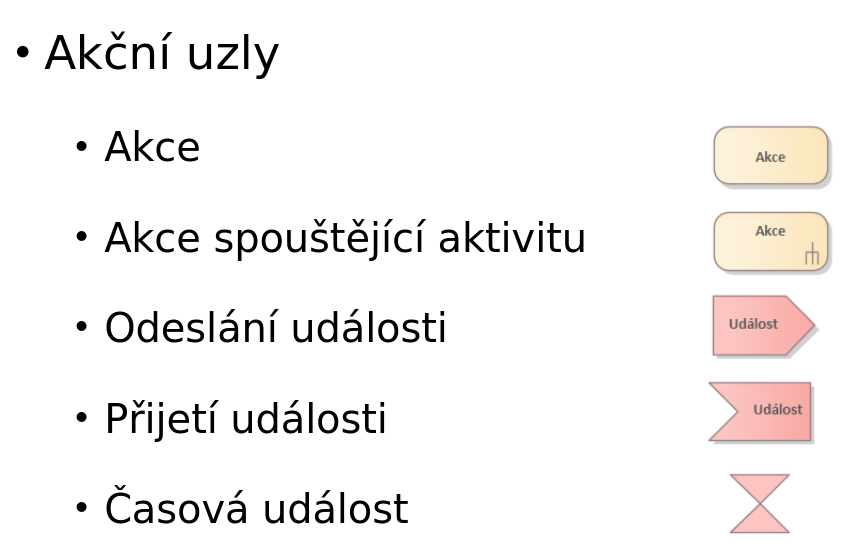
\includegraphics[width=0.8\textwidth]{img/screenshot_2025-05-12_15-27-12.png}
    \caption{Akční uzly}
    \label{fig:akcni_uzly}
\end{figure}

%screenshot_2025-05-12_15-29-42.png
\begin{figure}[H]
    \centering
    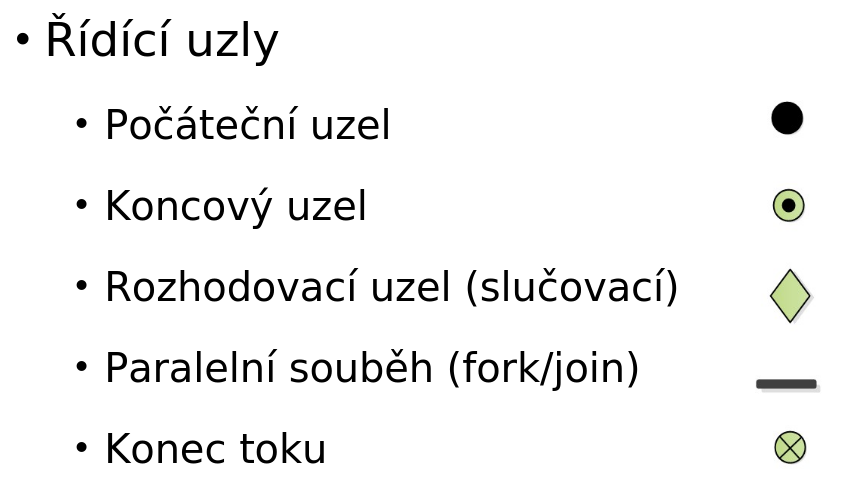
\includegraphics[width=0.8\textwidth]{img/screenshot_2025-05-12_15-29-42.png}
    \caption{Řídící uzly}
    \label{fig:ridici_uzly}
\end{figure}

%screenshot_2025-05-12_15-31-32.png
\begin{figure}[H]
    \centering
    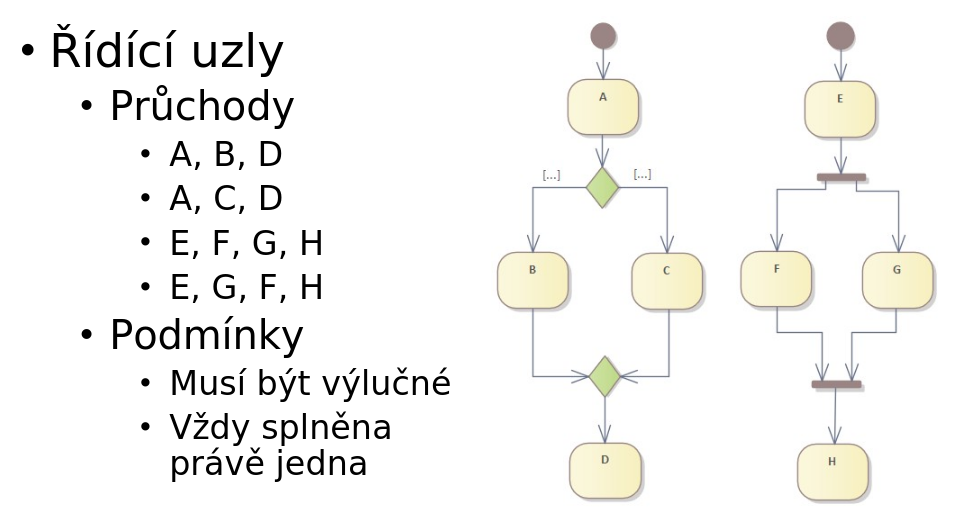
\includegraphics[width=0.8\textwidth]{img/screenshot_2025-05-12_15-31-32.png}
    \caption{Řídící uzly - průchod}
    \label{fig:ridici_uzly_pruchod}
\end{figure}

%screenshot_2025-05-12_15-32-22.png
\begin{figure}[H]
    \centering
    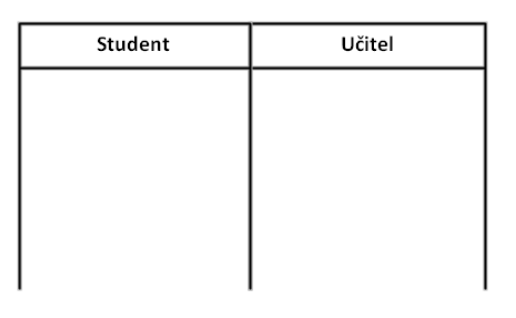
\includegraphics[width=0.8\textwidth]{img/screenshot_2025-05-12_15-32-22.png}
    \caption{Swimlanes - zóny zodpovědnosti}
    \label{fig:swimlanes}
\end{figure}

%screenshot_2025-05-12_15-36-12.png
\begin{figure}[H]
    \centering
    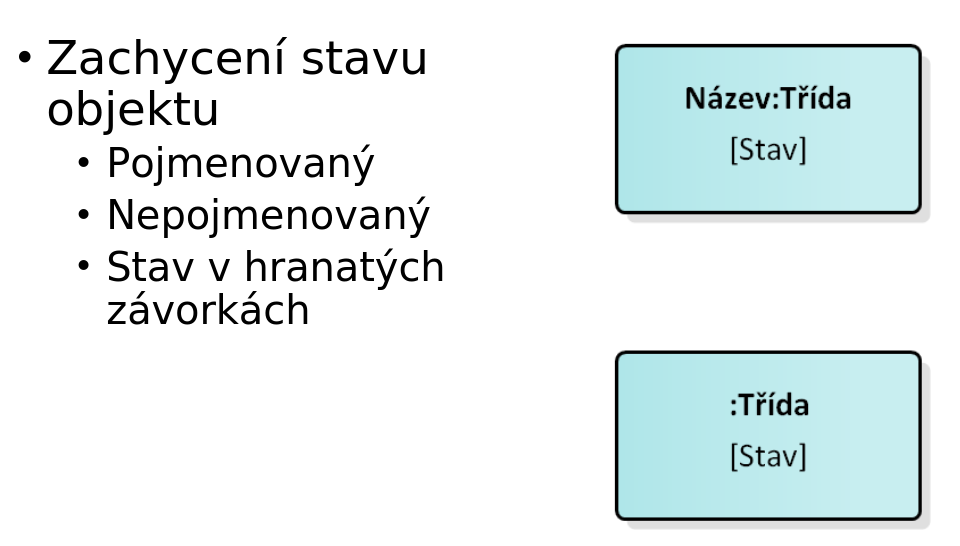
\includegraphics[width=0.8\textwidth]{img/screenshot_2025-05-12_15-36-12.png}
    \caption{Zachycení stavu}
    \label{fig:stavy}
\end{figure}

\subsubsection*{Analýza a správa požadavků}
\begin{itemize}
    \item Cíle
    \begin{itemize}
        \item Vymezit hranice systému
        \item Umožnit přesnější odhad pracnosti
        \item Vyjasnit si zadání s klientem
    \end{itemize}
    \item Kategorizace 
    \begin{itemize}
        \item Projektové (požadavky na cenu, termíny, kvalitu)
        \item Produktové
        \begin{itemize}
            \item Funkční (co konkrétně systém dělá)
            \item Nefunkční (obecné - výkon, použité standardy, omezení)
        \end{itemize}
    \end{itemize}
\end{itemize}

Produktové členění FURPS:
\begin{itemize}
    \item F (functionality) - funkčnost
    \item U (usability) - použitelnost
    \item R (reliability) - spolehlivost
    \item P (performance) - výkon
    \item S (supportability) - podpora / rozšířitelnost
\end{itemize}

\subsubsection*{Doménový model}

%screenshot_2025-05-13_12-10-53.png
\begin{figure}[H]
    \centering
    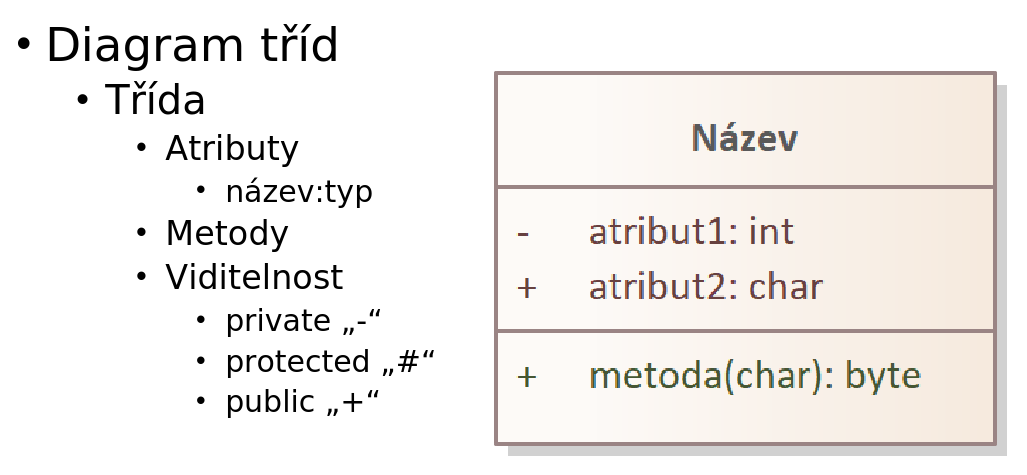
\includegraphics[width=0.8\textwidth]{img/screenshot_2025-05-13_12-10-53.png}
    \caption{Doménový model - entita}
    \label{fig:dom_model}
\end{figure}

%screenshot_2025-05-13_12-11-20.png
\begin{figure}[H]
    \centering
    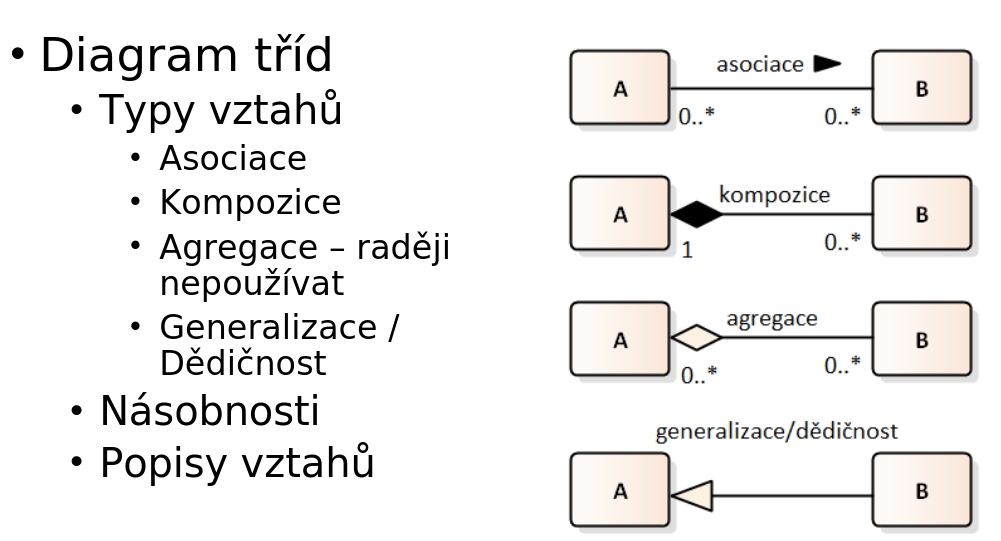
\includegraphics[width=0.8\textwidth]{img/screenshot_2025-05-13_12-11-20.png}
    \caption{Doménový model - vztahy}
    \label{fig:dom_model_priklad}
\end{figure}

Typy vztahů:
\begin{itemize}
    \item Asociace - stejný jako atribut, ale "čitelnější"
    \item Kompozice
    \item Agregace
    \item Generalizace (dědičnost)
\end{itemize}

\subsubsection*{UML stavový diagram}
%screenshot_2025-05-13_12-17-59.png

\begin{figure}[H]
    \centering
    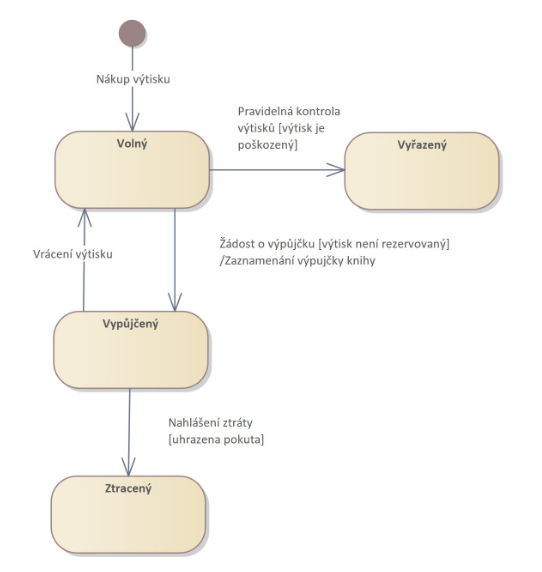
\includegraphics[width=0.8\textwidth]{img/screenshot_2025-05-13_12-17-59.png}
    \caption{UML stavový diagram}
    \label{fig:uml_stavovy_diagram}
\end{figure}
